% ============================================================
%  Chapter 12 — Software Tools and Emerging Technologies
%  for Vehicle Routing and Transportation
%  Source: Vehicle Routing: Problems, Methods, and Applications
%          2nd edition, 2014  (Toth & Vigo, eds.)
%  Chapter authors: Ola Braysy, Geir Hasle
% ============================================================
\documentclass[aspectratio=169,10pt]{beamer}
\usetheme{Madrid}
\usecolortheme{seahorse}

% ---- packages -------------------------------------------------------
\usepackage{amsmath,amssymb,amsfonts}
\usepackage{booktabs}
\usepackage{graphicx}
\usepackage{xcolor}
\usepackage{listings}
\usepackage{array}
\usepackage{multirow}
\usepackage{hyperref}
\usepackage{microtype}
\usepackage{lmodern}
\usepackage{textcomp}

% ---- graphics path --------------------------------------------------
\graphicspath{{figures/}}

% ---- listings style -------------------------------------------------
\lstset{
  language=Python,
  basicstyle=\ttfamily\scriptsize,
  numbers=left,
  numberstyle=\tiny\color{gray},
  stepnumber=1,
  frame=single,
  backgroundcolor=\color{gray!7},
  commentstyle=\color{green!50!black}\itshape,
  keywordstyle=\color{blue!70!black}\bfseries,
  stringstyle=\color{orange!80!black},
  breaklines=true,
  showstringspaces=false,
  tabsize=4,
}

% ---- footer ---------------------------------------------------------
\setbeamertemplate{footline}[frame number]
\setbeamertemplate{navigation symbols}{}

% ---- title page data ------------------------------------------------
\title[Ch.\ 12: VRP Software \& Emerging Tech]{%
  \textbf{Chapter 12}\\
  Software Tools and Emerging Technologies\\
  for Vehicle Routing and Transportation}
\subtitle{Vehicle Routing: Problems, Methods, and Applications, 2nd ed.\ (2014)}
\author{Based on: Ola Brays{\o}y \& Geir Hasle}
\institute{Slides prepared for self-contained study}
\date{2026}

% ====================================================================
\begin{document}
% ====================================================================

\begin{frame}
  \titlepage
\end{frame}

% ----------------------------------------------------------------
\begin{frame}[allowframebreaks]{Chapter Overview}
  This chapter surveys the \textbf{software landscape} for Vehicle Routing Problems
  (VRPs): what commercial and open-source tools exist, what algorithmic engines they
  use, how they handle data and user interaction, and where the technology is heading.

  \tableofcontents[hideallsubsections]
\end{frame}

\AtBeginSection[]{%
  \begin{frame}[allowframebreaks]{Outline}
    \tableofcontents[currentsection, hideallsubsections]
  \end{frame}
}

% ====================================================================
\section{Introduction}
% ====================================================================

\begin{frame}[allowframebreaks]{12.1 \; Introduction}
  Vehicle routing is a central problem for a large number of public and private
  corporations, including logistics companies, parcel delivery services, transit
  agencies, and solid-waste collection firms.
  Solving real VRP instances well can cut transport costs by \textbf{5--30\%},
  reduce fuel consumption and CO$_2$ emissions, and improve customer service levels.

  \begin{block}{Why software matters more than algorithms alone}
    The academic literature has produced dozens of powerful exact methods,
    heuristics, and metaheuristics for VRP.
    However, a mathematical algorithm by itself is not directly useful to a
    practitioner: it must be embedded in a \emph{software product} that:
    \begin{itemize}
      \item reads real-world problem data (addresses, time windows, vehicle specs),
      \item integrates with mapping and GIS (Geographic Information System) layers,
      \item enforces dozens of practical business constraints,
      \item presents routes to planners and drivers in an understandable form, and
      \item can be maintained and extended over time.
    \end{itemize}
  \end{block}

  \framebreak

  \begin{alertblock}{The gap between research and practice}
    Research algorithms are often developed and tested on \emph{benchmark instances}
    (e.g., Solomon's 100-customer VRPTW instances) under idealised assumptions.
    Real-world deployments involve:
    \begin{itemize}
      \item thousands of customers per day,
      \item dozens of interacting constraints (driver breaks, hazmat, vehicle
            compatibility, customer preferences),
      \item uncertain travel times (traffic), dynamic new orders, and
      \item the need for human planners to understand, trust, and override
            the software.
    \end{itemize}
    Bridging this gap is the central challenge of \emph{VRP software technology}.
  \end{alertblock}

  \medskip
  This chapter focuses on \textbf{applied} aspects: it does not present new
  algorithms, but instead analyses how the best existing algorithms are
  integrated into commercial products and what practical requirements drive
  software design decisions.

  \framebreak

  \begin{block}{Scope of the survey}
    The authors conducted a questionnaire-based survey of VRP software vendors,
    receiving responses from nine companies operating worldwide
    (Table 12.1, discussed in Section 12.7).
    The survey covered:
    \begin{enumerate}
      \item system architecture and user interfaces,
      \item input/output capabilities and data integration,
      \item supported VRP model variants,
      \item embedded algorithms and solvers,
      \item implementation platform, performance benchmarks, and pricing, and
      \item adoption of emerging technologies.
    \end{enumerate}
    The chapter also reviews the open-source and academic software landscape
    and discusses future directions.
  \end{block}

  \begin{alertblock}{Key insight: industrial VRP is complex}
    Vendors report that the typical industrial VRP involves far more than distance
    minimisation: the problem includes driver working-hour regulations, vehicle
    compatibility rules, geographic zoning, multi-day planning horizons, and
    real-time order changes.
    A routing algorithm that cannot handle these aspects cannot be deployed in
    practice, regardless of its theoretical performance.
  \end{alertblock}
\end{frame}

% ====================================================================
\section{Basic Functionalities of VRP Software}
% ====================================================================

\begin{frame}[allowframebreaks]{12.2 \; Basic Functionalities of VRP Routing Software}

  Every VRP software product, whether commercial or open-source, must provide
  a core set of functionalities.
  Understanding these functionalities helps us evaluate and compare tools.

  \begin{block}{Core components of a VRP routing system}
    A routing system typically comprises four main modules:
    \begin{enumerate}
      \item \textbf{GIS (Geographic Information System) Module} ---
            integrates map data, computes travel times and distances between
            locations, geocodes addresses (converts street addresses to
            latitude/longitude coordinates).
      \item \textbf{Problem Data Module} ---
            stores and manages customer data (locations, demands, time windows,
            priorities), vehicle data (capacity, type, availability), and
            depot information.
      \item \textbf{Optimization Module} ---
            the algorithmic engine that computes routes; may include
            construction heuristics, local search, metaheuristics, or
            exact solvers.
      \item \textbf{Output/Reporting Module} ---
            displays routes on maps, generates driver turn-by-turn directions,
            exports data to ERP (Enterprise Resource Planning) and TMS
            (Transport Management System) systems, and computes KPIs
            (Key Performance Indicators) such as total distance, cost, and
            service level.
    \end{enumerate}
  \end{block}

  \framebreak

  \begin{figure}
    \centering
    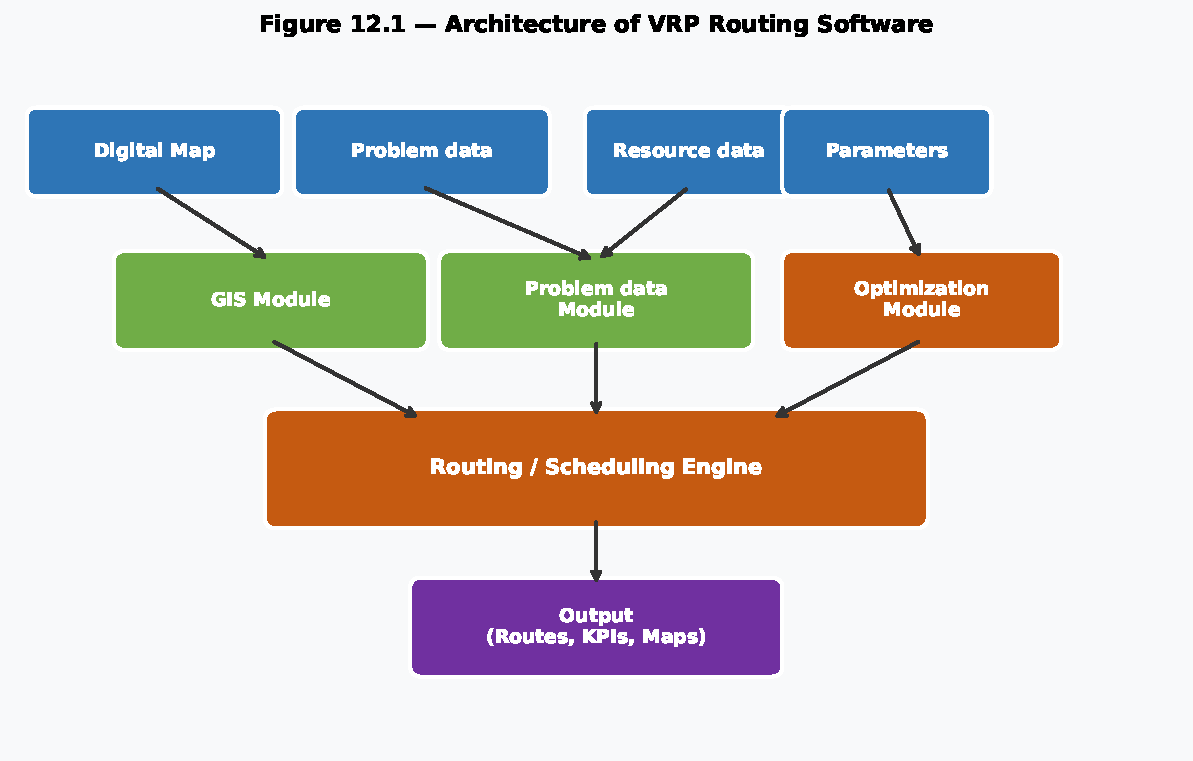
\includegraphics[width=0.85\textwidth]{fig_software_architecture.pdf}
    \caption{Architecture of a typical VRP routing software system.
             Data flows from inputs (digital map, problem data, resources, parameters)
             through the GIS and problem-data modules into the routing engine,
             and results are delivered as routes, maps, and performance reports.}
  \end{figure}

  \framebreak

  \begin{block}{The routing engine in detail}
    The \textbf{routing engine} (also called the \emph{optimization engine} or
    \emph{solver}) is the intellectual core of the system.
    It receives:
    \begin{itemize}
      \item a \emph{distance/time matrix}: an $n \times n$ table where entry
            $(i,j)$ gives the travel time (or distance) from location $i$ to
            location $j$ --- here $n$ (read: ``n'') is the total number of
            locations including the depot and all customers,
      \item resource data (vehicle capacities, driver shift lengths), and
      \item constraint parameters (time windows, required vehicle types).
    \end{itemize}
    It returns a \emph{set of routes} --- one per vehicle --- each specifying the
    order in which customers are visited.
  \end{block}

  \begin{block}{Planning modes}
    Most systems support three planning horizons:
    \begin{itemize}
      \item \textbf{Tactical/strategic planning} --- optimise routes for a
            typical or average day; used for contract design and fleet sizing.
      \item \textbf{Operational planning} --- day-to-day route optimisation
            run the evening before, incorporating the actual next-day orders.
      \item \textbf{Real-time/dynamic replanning} --- adjust routes during
            the day as new orders arrive, vehicles deviate from schedule,
            or unexpected events occur (traffic jams, breakdowns).
    \end{itemize}
  \end{block}

  \framebreak

  \begin{block}{A planning module model for VRP software (Figure 12.1)}
    According to the taxonomy used in the book, planning modules include:
    \begin{itemize}
      \item an \textbf{interface} to the GIS system for distances, times,
            and map display;
      \item a \textbf{GIS module} for geocoding, routing, and map integration;
      \item a \textbf{problem data module} for customer, vehicle, and depot data;
      \item a \textbf{planning module} for automated and manual route construction,
            providing for multi-period planning;
      \item a \textbf{statistics module} for performance indicators and reports; and
      \item a \textbf{simulation module} to test what-if scenarios.
    \end{itemize}
  \end{block}

  \begin{alertblock}{Key insight}
    The quality of a VRP software product depends not only on the optimization
    algorithm but equally on the completeness and correctness of its constraint
    model, the richness of its GIS integration, and the usability of its
    interface for human planners.
  \end{alertblock}
\end{frame}

% ====================================================================
\section{Input and Output}
% ====================================================================

\begin{frame}[allowframebreaks]{12.3 \; Input and Output}

  A VRP system must be able to read data from the user's existing IT
  infrastructure and return results in formats that integrate with downstream
  systems.
  Poor I/O capabilities are often a bigger barrier to adoption than algorithmic
  limitations.

  \begin{block}{Typical input data formats}
    \begin{itemize}
      \item \textbf{Spreadsheets} (CSV, Excel) --- the most common entry
            point for smaller operations; customer lists with addresses,
            demands, and time windows.
      \item \textbf{ERP/TMS system integration} --- via APIs, ODBC/JDBC
            database connections, or XML/JSON feeds from systems such as
            SAP, Oracle, or Microsoft Dynamics.
      \item \textbf{EDI (Electronic Data Interchange)} --- standardised
            electronic business documents (orders, invoices) in formats
            such as EDIFACT or ANSI X12.
      \item \textbf{GPS track logs} --- historical vehicle positions in
            formats such as NMEA, GPX, or vendor-specific binary formats;
            used for driver performance analysis and model calibration.
    \end{itemize}
  \end{block}

  \framebreak

  \begin{block}{Map and GIS data}
    A routing system needs a \emph{road network} to compute realistic travel
    times and distances.
    Sources include:
    \begin{itemize}
      \item \textbf{Commercial digital maps} --- HERE (formerly Navteq),
            TomTom, Google Maps Platform; typically licensed annually.
            Provide turn restrictions, road speeds, truck-height
            restrictions, etc.
      \item \textbf{OpenStreetMap (OSM)} --- free, crowd-sourced global
            map; quality varies by region; sufficient for many applications.
      \item \textbf{Proprietary road-speed databases} --- some vendors
            combine map data with historical GPS probe data to provide
            time-of-day-dependent travel times (e.g., faster at 2 am
            than at 8 am rush hour).
    \end{itemize}
  \end{block}

  \begin{block}{Geocoding}
    \textbf{Geocoding} is the process of converting a street address such as
    ``75 Port-Royal Street East, Montreal'' into geographic coordinates
    (latitude, longitude).
    Accurate geocoding is essential: a geocoding error of even 100~metres
    can cause the system to assign a customer to the wrong road segment,
    leading to incorrect travel times and infeasible routes.
    Most commercial systems include or interface with a geocoding service.
  \end{block}

  \framebreak

  \begin{figure}
    \centering
    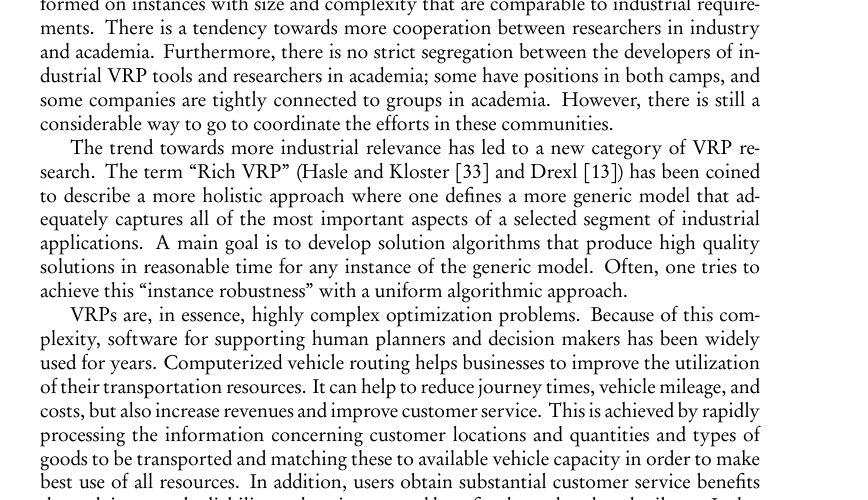
\includegraphics[width=0.78\textwidth]{fig_book_fig12_1.png}
    \caption{Screenshot of a typical VRP routing software interface
             (Figure 12.2 from the book).
             The map view shows planned routes superimposed on a road network,
             with coloured route segments and depot/customer markers.
             Adjacent panels allow the planner to inspect individual route
             details and edit assignments manually.}
  \end{figure}

  \framebreak

  \begin{block}{Output: what the system delivers}
    \begin{itemize}
      \item \textbf{Route lists} --- ordered sequences of stops for each
            driver, with estimated arrival/departure times at each stop.
      \item \textbf{Map visualisation} --- routes drawn on a map for
            planner review and manual adjustment.
      \item \textbf{Driver manifests} --- printed or electronic documents
            given to drivers: customer name, address, delivery quantity,
            time window, and special instructions.
      \item \textbf{KPI reports} --- total distance, total time, vehicle
            utilisation (load percentage), number of vehicles used,
            estimated fuel cost, CO$_2$ emissions.
      \item \textbf{Export to downstream systems} --- route data pushed back
            to TMS, WMS (Warehouse Management System), or billing systems.
      \item \textbf{Mobile/GPS dispatch} --- routes transmitted directly to
            in-vehicle navigation devices or driver smartphones.
    \end{itemize}
  \end{block}

  \begin{alertblock}{Key insight}
    Software usability for the planner is as important as solution quality.
    Planners must be able to override automated routes, add or remove stops,
    and reoptimise quickly.
    Systems that are difficult to use tend to be abandoned in favour of
    manual planning --- even if their algorithmic solutions are better.
  \end{alertblock}
\end{frame}

% ====================================================================
\section{Model Properties}
% ====================================================================

\begin{frame}[allowframebreaks]{12.4 \; Model Properties --- Supported VRP Variants}

  A VRP software product is only useful if it can model the constraints
  that arise in the user's actual operations.
  This section surveys the main constraint types supported by commercial tools.

  \begin{block}{12.4.1 \; Basic setup: order types}
    The most fundamental choice is the \textbf{order type}:
    \begin{itemize}
      \item \textbf{Pickup-only} (e.g., collecting goods from suppliers).
      \item \textbf{Delivery-only} (e.g., delivering parcels from depot
            to customers) --- the most common case.
      \item \textbf{Mixed pickup and delivery} --- vehicles collect goods
            from some locations and deliver to others; the two types may
            be interleaved on the same route.
        \begin{itemize}
          \item \emph{Simultaneous pickup and delivery (SPDP)}: at each
                customer the driver both delivers and picks up.
          \item \emph{Paired pickup-and-delivery (PDP)}: each pickup
                location is paired with a specific delivery location
                (e.g., courier, dial-a-ride).
        \end{itemize}
    \end{itemize}
  \end{block}

  \framebreak

  \begin{block}{Route start and end flexibility}
    In the classical VRP, all vehicles start and end at the same depot.
    Real operations often require:
    \begin{itemize}
      \item \textbf{Multiple depots} --- several warehouses or terminals.
      \item \textbf{Open routes} --- vehicles end at their last customer
            (driver goes home) rather than returning to the depot.
      \item \textbf{Multiple time horizons} ---
            routes spanning several days, e.g., long-haul trucking.
    \end{itemize}
  \end{block}

  \begin{block}{Planning Horizon}
    One frequently encountered complication is that planning must be done
    over more than a single day.
    For example, a wholesale distributor may visit some customers only on
    Mondays and Wednesdays, others on Tuesdays and Thursdays.
    This leads to \textbf{period VRP} variants, supported by several
    commercial systems.
  \end{block}

  \framebreak

  \begin{block}{12.4.2 \; Uncertainty and Dynamics}

    \textbf{Uncertainty.}
    Real customer demands are often not known exactly in advance.
    A system must handle:
    \begin{itemize}
      \item \emph{Stochastic demands} --- the actual demand at customer $i$
            is a random variable $\tilde{d}_i$ (d-tilde sub $i$) with
            known probability distribution; the route must be feasible
            with high probability.
      \item \emph{Dynamic orders} --- new customer orders arrive during the
            planning day and must be inserted into existing routes.
    \end{itemize}

    \textbf{Delivery Day.}
    Some customers require delivery on a specific day or on one of several
    allowed days.
    For example, a dairy product may need to be delivered within 24 hours of
    order.

    \textbf{Priorities.}
    In practice, customers differ in importance.
    Priority constraints allow the planner to specify that high-priority
    customers must be served first or within a tighter time window.
    Some tools support \emph{soft} priorities that can be violated at a penalty cost.
  \end{block}

  \framebreak

  \begin{block}{Same-Tour Constraints and Time Limits}
    \textbf{Same-Tour Constraints.}
    Some business rules require that:
    \begin{itemize}
      \item certain customers always travel on the \emph{same} route (same vehicle),
            e.g., hazmat customers grouped with a certified driver; or
      \item certain customers must \emph{never} be on the same route
            (competing customers who must not see each other's orders).
    \end{itemize}

    \textbf{Time Limits.}
    Maximum route duration (total time on road) and maximum shift length
    for drivers are standard constraints.
    Some systems also support:
    \begin{itemize}
      \item mandatory rest breaks (e.g., EU regulations require a 45-minute
            break after 4.5 hours of driving),
      \item overtime rules and associated cost penalties.
    \end{itemize}
  \end{block}

  \framebreak

  \begin{block}{Time Windows (VRPTW)}
    Time windows are among the most commonly used and most impactful
    constraints in real VRP applications.

    A \textbf{time window} $[a_i, b_i]$ for customer $i$ specifies that
    service must begin no earlier than time $a_i$ (a sub $i$, the
    \emph{opening time}) and no later than time $b_i$ (b sub $i$, the
    \emph{closing time}).
    Here $a$ and $b$ are typically given in minutes or hours from
    the start of the planning horizon (e.g., 08:00 = 0, 09:00 = 60).

    \begin{itemize}
      \item \emph{Hard time windows}: arriving after $b_i$ is infeasible;
            the customer cannot be served.
      \item \emph{Soft time windows}: arriving after $b_i$ incurs a penalty
            cost proportional to the lateness $\max(0,\, t_i - b_i)$,
            where $t_i$ (t sub $i$) is the actual arrival time.
    \end{itemize}
    Most commercial tools support both hard and soft time windows.
  \end{block}

  \begin{figure}
    \centering
    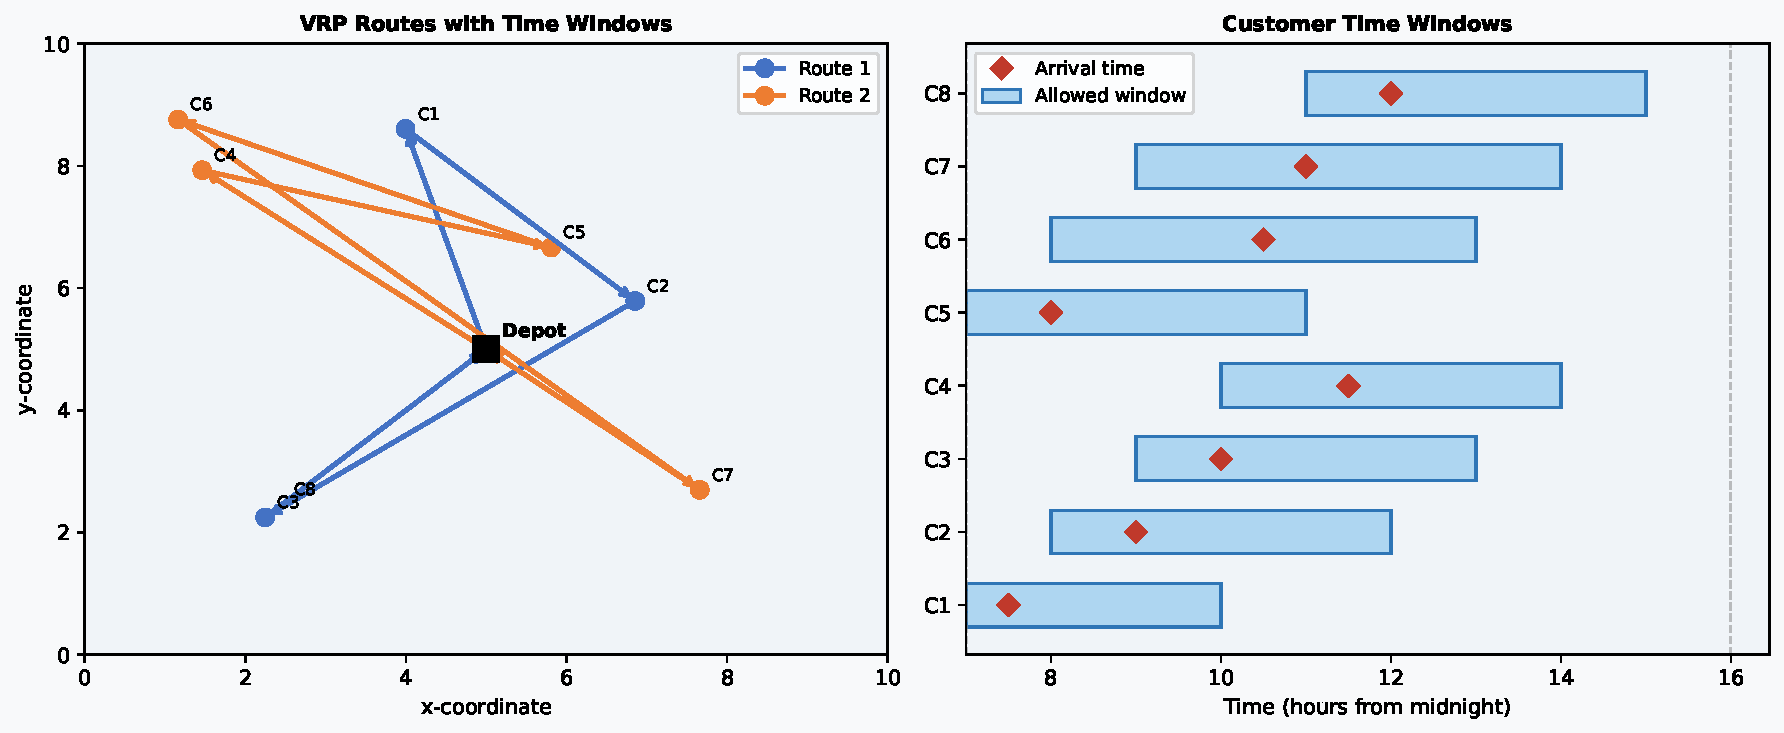
\includegraphics[width=0.85\textwidth]{fig_time_window.pdf}
    \caption{Left: two optimised routes for 8 customers.
             Right: each customer's allowed delivery window (blue bar)
             and the planned arrival time (red diamond).
             All arrivals fall within the windows in this example.}
  \end{figure}

  \framebreak

  \begin{block}{Capacity Constraints}
    The most basic VRP constraint is vehicle \textbf{capacity}:
    the total load carried on a route must not exceed the vehicle's
    maximum capacity $Q$ (Q, a positive number representing
    weight, volume, or number of items).

    Many real applications involve \emph{multiple capacity types}
    simultaneously.
    For example, a food-distribution vehicle may be limited by:
    \begin{itemize}
      \item \emph{weight} (e.g., maximum 5 tonnes),
      \item \emph{volume} (e.g., maximum 20 cubic metres), and
      \item \emph{number of pallets} (e.g., maximum 33 Euro-pallets).
    \end{itemize}
    All three constraints must hold simultaneously.

    Most commercial VRP systems support multiple capacity dimensions.
    Open-source systems often support only a single dimension.
  \end{block}

  \begin{block}{Temporal Availability}
    Customers, drivers, and vehicles may each have \emph{availability windows}:
    time intervals during which they can participate in a route.
    A vehicle may be available only from 06:00 to 22:00;
    a driver may work only a morning or afternoon shift.
    These constraints interact with time windows to make the feasibility
    check non-trivial.
  \end{block}

  \framebreak

  \begin{block}{Compatibility Constraints}
    In many industries, not every vehicle can serve every customer:
    \begin{itemize}
      \item A \emph{refrigerated truck} is required for temperature-sensitive goods.
      \item A \emph{tail-lift vehicle} is needed for customers without
            loading docks.
      \item A \emph{certified hazmat vehicle and driver} are legally required
            for dangerous goods.
      \item \emph{Vehicle size restrictions} apply on narrow roads or in
            pedestrian zones.
    \end{itemize}
    These are modelled as \textbf{compatibility matrices}: a binary table
    specifying which (vehicle, customer) pairs are compatible.
  \end{block}

  \begin{block}{Driving Regulations}
    European and North American regulations impose mandatory rest periods.
    The EU drivers' hours rules (Regulation (EC) No 561/2006) state:
    \begin{itemize}
      \item After 4.5 hours of continuous driving, a 45-minute break is required.
      \item The daily driving limit is 9 hours (extendable to 10 hours twice a week).
      \item 11 hours of daily rest are mandatory.
    \end{itemize}
    Commercial VRP software must model these rules and insert required
    breaks at feasible locations on each route.
    Only a few systems handle this fully.
  \end{block}

  \framebreak

  \begin{block}{Zoning}
    \textbf{Zoning} refers to geographic or administrative groupings that
    constrain how customers are assigned to vehicles or routes:
    \begin{itemize}
      \item \emph{Predefined service zones} --- a delivery region is divided
            into zones, each assigned to a specific vehicle or driver.
            Useful for driver familiarity and customer relationship management.
      \item \emph{Zone balancing} --- the system aims to keep zones roughly
            equal in workload across multiple planning periods.
      \item \emph{Zone optimisation} --- the system redesigns zone boundaries
            along with routes, a more powerful but computationally harder approach.
    \end{itemize}
  \end{block}

  \begin{figure}
    \centering
    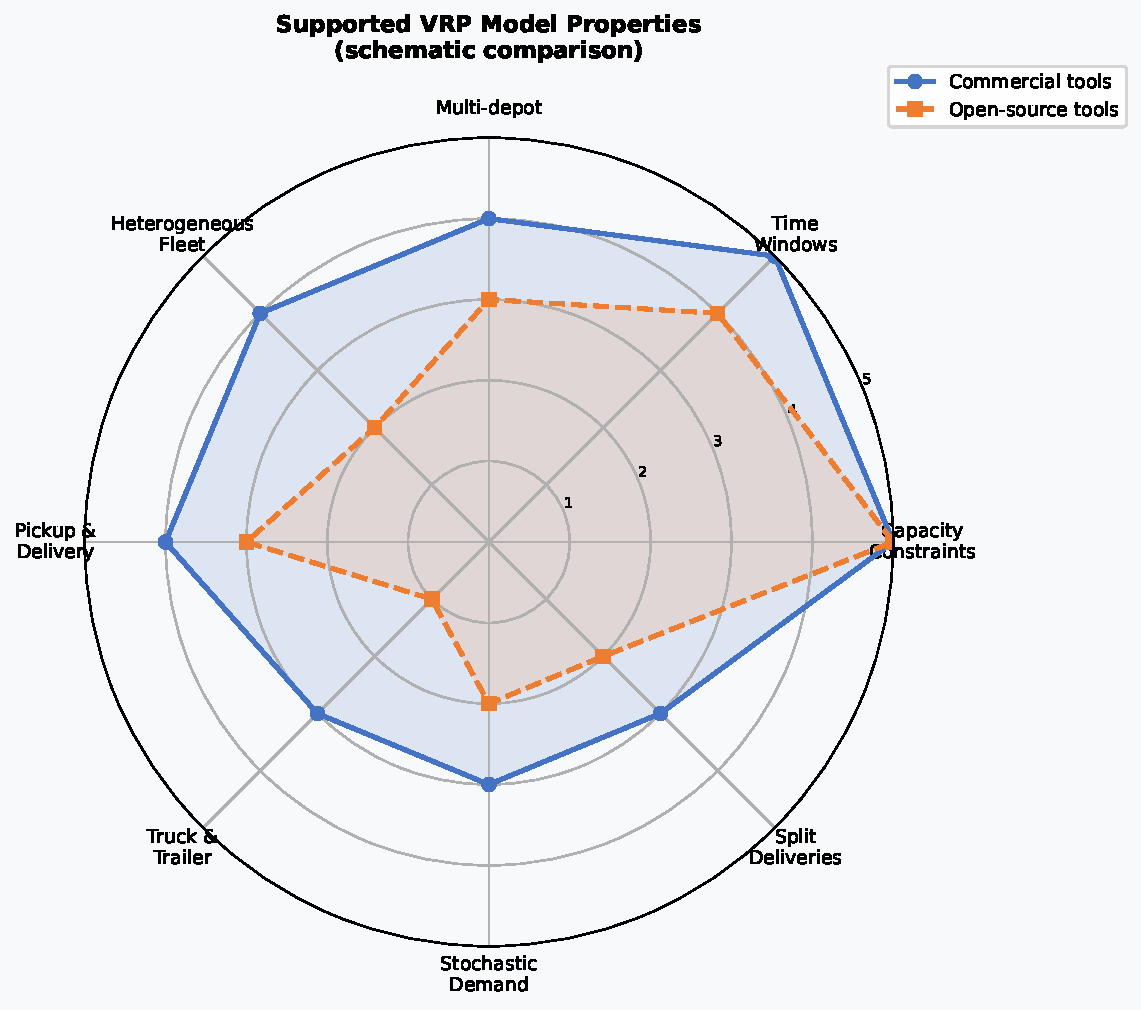
\includegraphics[width=0.72\textwidth]{fig_model_properties.pdf}
    \caption{Schematic comparison of model property coverage between
             commercial and open-source VRP tools.
             Commercial tools (blue) generally support a broader range of
             constraint types, particularly for stochastic demands and
             truck-and-trailer routing.}
  \end{figure}
\end{frame}

% ====================================================================
\section{Algorithms}
% ====================================================================

\begin{frame}[allowframebreaks]{12.5 \; Algorithms in Commercial VRP Software}

  Information on the algorithms used inside commercial VRP tools is usually
  not publicly disclosed, as it is a proprietary asset.
  However, the survey results and published research allow some conclusions.
  The dominant methods in commercial systems are \textbf{metaheuristics},
  with some exact methods for small sub-problems.

  \begin{block}{Most common algorithmic strategies}
    \begin{enumerate}
      \item \textbf{Construction heuristics} --- build an initial feasible
            solution quickly (seconds or less), even if suboptimal.
            Used as a starting point for improvement.
            Examples: Clarke-Wright Savings, Nearest Neighbour insertion,
            Sweep algorithm.

      \item \textbf{Local search / improvement heuristics} ---
            iteratively improve the current solution by making small changes
            (moves).
            A move is accepted if it reduces the objective (total distance/cost).
            Terminates at a local minimum.
            Examples: 2-opt, 3-opt, Or-opt (relocate one or two customers).

      \item \textbf{Metaheuristics} --- sophisticated search strategies that
            can escape local minima by sometimes accepting worse solutions
            or by exploring multiple solutions simultaneously.
            Examples: Tabu Search, Simulated Annealing, Genetic Algorithms,
            ALNS (Adaptive Large Neighbourhood Search).

      \item \textbf{Exact methods} --- solve a mathematical programming
            formulation to provable optimality; practical only for
            small instances (up to $\sim$100 customers) or small
            sub-problems.
            Examples: Branch-and-Bound, Branch-and-Cut, Column Generation.
    \end{enumerate}
  \end{block}

  \framebreak

  \begin{figure}
    \centering
    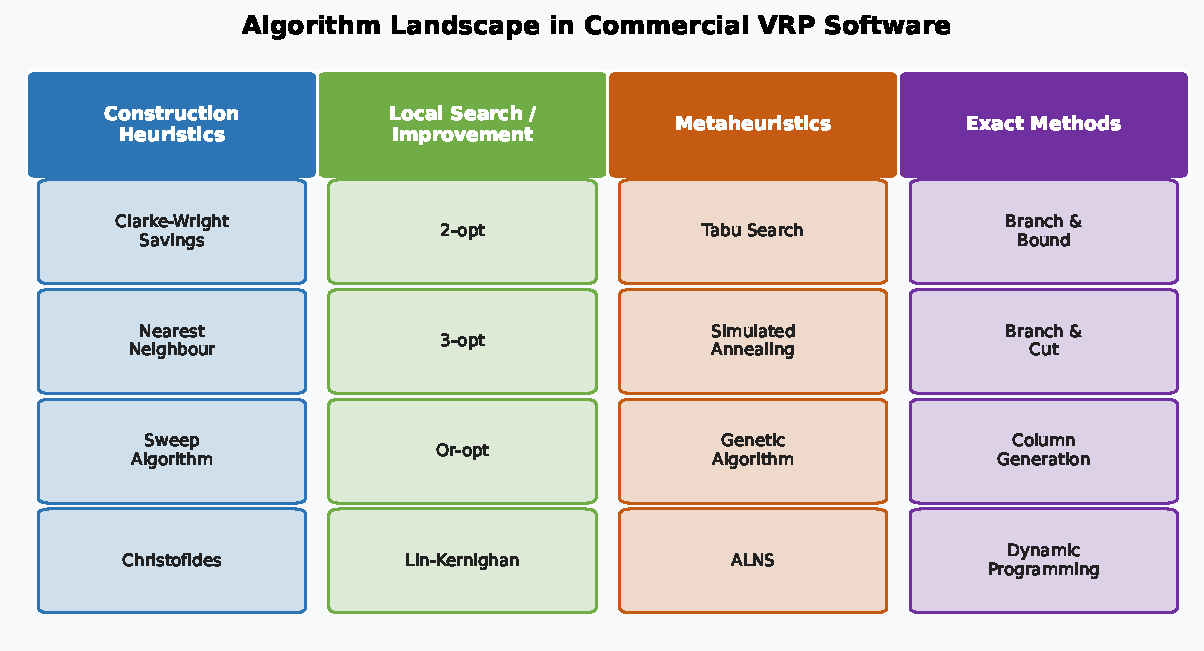
\includegraphics[width=0.88\textwidth]{fig_algorithm_landscape.pdf}
    \caption{The algorithm landscape in commercial VRP software.
             Construction heuristics provide a fast starting point;
             local search improves it; metaheuristics enable large-scale
             high-quality optimisation; and exact methods provide
             optimal solutions for small instances.}
  \end{figure}

  \framebreak

  \begin{block}{The Clarke-Wright Savings Algorithm (1964)}
    This is the most widely used construction heuristic for VRP and is
    included in almost every commercial system.
    The central idea is that it is cheaper to serve two customers $i$ and $j$
    on the \emph{same} route than on two separate routes, whenever their
    locations are close to each other relative to the depot.

    \textbf{The saving} of merging customers $i$ and $j$ onto a single route is:
    \[
      s(i,j) \;=\; d_{0i} + d_{0j} - d_{ij}
    \]
    where:
    \begin{itemize}
      \item $d_{0i}$ (d sub 0,i) = distance from depot (node 0) to customer $i$,
      \item $d_{0j}$ (d sub 0,j) = distance from depot to customer $j$, and
      \item $d_{ij}$ (d sub i,j) = distance from customer $i$ to customer $j$.
    \end{itemize}
    If $s(i,j) > 0$ (positive saving), combining the two stops saves distance
    compared to visiting each customer on a separate trip.
  \end{block}

  \begin{alertblock}{How to read this formula}
    Think of it this way: the original cost of two separate out-and-back trips
    is $2d_{0i} + 2d_{0j}$ (depot$\to i\to$depot, then depot$\to j\to$depot).
    If we merge them into one route (depot$\to i\to j\to$depot), the cost
    becomes $d_{0i} + d_{ij} + d_{0j}$.
    The saving is the difference: $d_{0i} + d_{0j} - d_{ij}$.
    A larger saving means combining $i$ and $j$ gives a bigger distance
    reduction.
  \end{alertblock}

  \framebreak

  \begin{exampleblock}{Worked Example: Clarke-Wright with 5 Customers}
    Consider a depot at the origin $(0,0)$ and five customers at coordinates:
    $C_1=(2,3)$, $C_2=(4,1)$, $C_3=(5,4)$, $C_4=(1,5)$, $C_5=(6,2)$.
    (All distances are Euclidean.)

    \textbf{Step 1: compute distances from depot.}
    \[
      d_{01} = \sqrt{2^2+3^2} \approx 3.61, \quad
      d_{02} = \sqrt{4^2+1^2} \approx 4.12, \quad
      d_{03} \approx 6.40, \quad
      d_{04} \approx 5.10, \quad
      d_{05} \approx 6.32.
    \]

    \textbf{Step 2: compute top savings.}
    \[
      s(3,5) = 6.40 + 6.32 - d_{35} \approx 12.72 - \sqrt{1+4} \approx 12.72 - 2.24 = 10.48
    \]
    \[
      s(1,4) = 3.61 + 5.10 - \sqrt{1+4} \approx 8.71 - 2.24 = 6.47
    \]

    \textbf{Step 3: merge in savings order (subject to capacity).}
    Start with 5 individual routes.
    Merge $C_3$ and $C_5$ first (largest saving): route becomes
    depot$\to C_3 \to C_5\to$depot.
    Then merge $C_1$ and $C_4$: depot$\to C_1 \to C_4\to$depot.
    $C_2$ remains on its own route if capacity is exhausted.

    \textbf{Result:} 3 routes; total distance reduced by approximately
    $10.48 + 6.47 = 16.95$ units compared to 5 individual trips.
  \end{exampleblock}

  \framebreak

  \begin{figure}
    \centering
    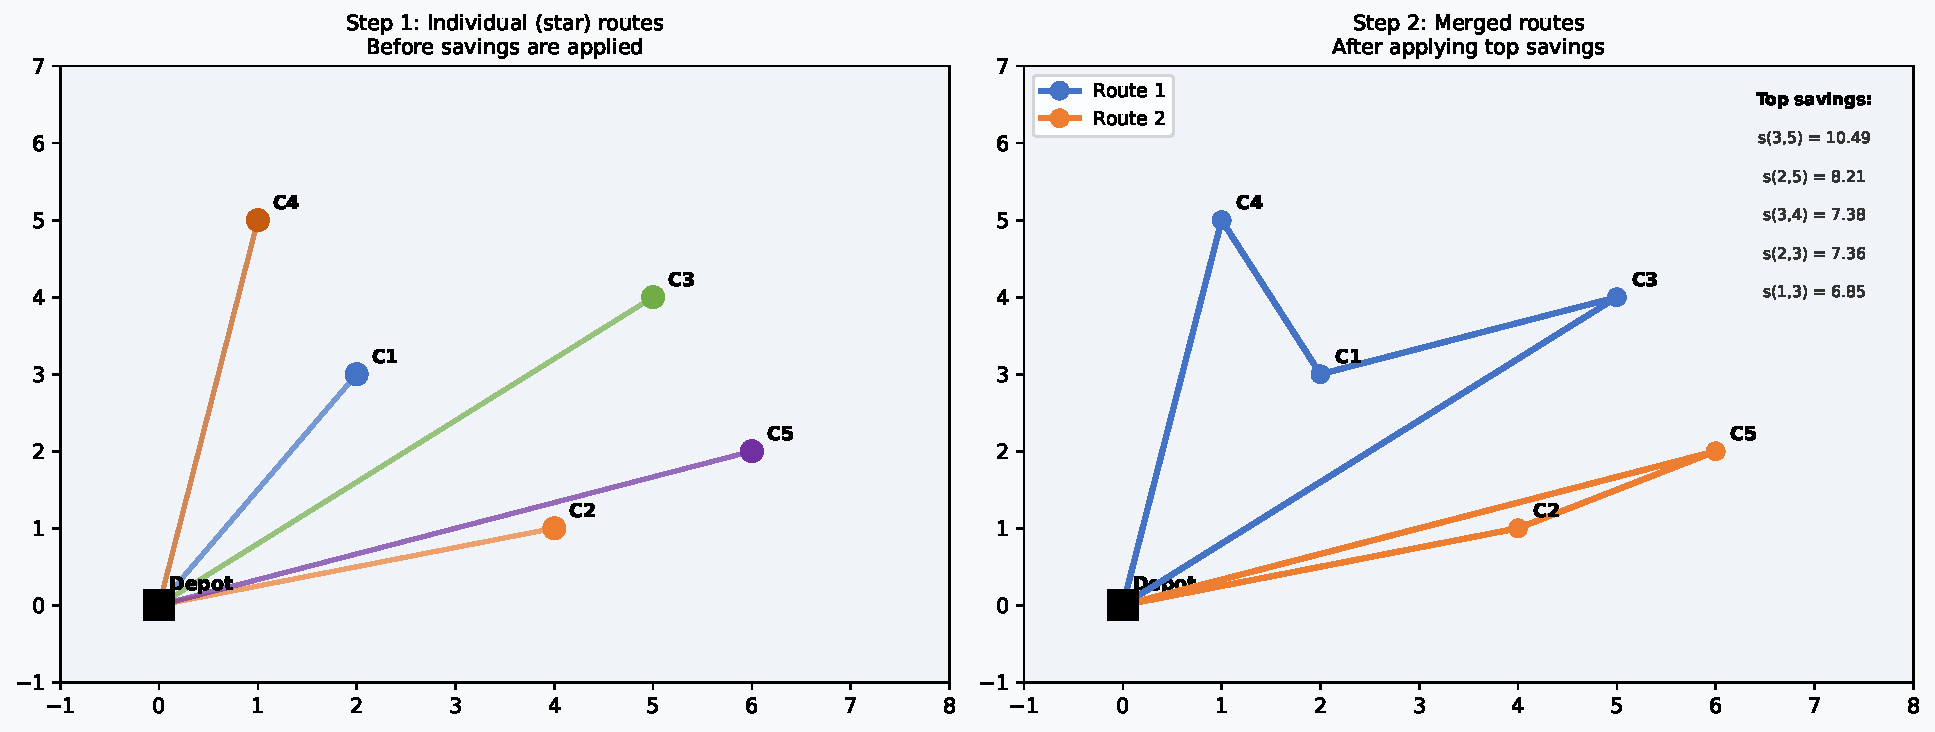
\includegraphics[width=0.88\textwidth]{fig_clarke_wright.pdf}
    \caption{Clarke-Wright algorithm illustration.
             Left: the initial ``star'' configuration with one separate
             out-and-back trip per customer.
             Right: after applying the top savings, customers are merged
             into two routes (blue and orange), significantly reducing
             total travel distance.}
  \end{figure}

  \framebreak

  \begin{block}{Clarke-Wright: Pseudocode (Parallel Version)}
    \begin{enumerate}
      \item \textbf{Initialise}: create $n$ individual routes, one per customer:
            route$_i$ = (depot $\to$ customer$_i$ $\to$ depot).
      \item \textbf{Compute savings}: for all pairs $(i,j)$ with $i \neq j$,
            compute $s(i,j) = d_{0i} + d_{0j} - d_{ij}$.
      \item \textbf{Sort}: order all pairs by decreasing savings.
      \item \textbf{Merge greedily}: for each pair $(i,j)$ in sorted order:
        \begin{enumerate}
          \item[(4a)] Check if $i$ is at the \emph{end} of its current route
                     and $j$ is at the \emph{beginning} of its current route
                     (or vice versa), and the two routes are different.
          \item[(4b)] Check that merging does not violate the capacity constraint:
                     combined load $\leq Q$.
          \item[(4c)] If both checks pass, merge the two routes into one.
        \end{enumerate}
      \item \textbf{Return} the set of routes.
    \end{enumerate}
  \end{block}

  \begin{alertblock}{Complexity}
    Computing all savings takes $O(n^2)$ time (order $n$-squared).
    Sorting takes $O(n^2 \log n)$.
    The greedy merge loop is at most $O(n^2)$ iterations.
    Total: $O(n^2 \log n)$ --- fast even for thousands of customers.
  \end{alertblock}

  \framebreak

  \begin{block}{Tabu Search: the core idea}
    \textbf{Tabu Search} (TS) is a local search method that avoids cycling
    by maintaining a \emph{tabu list} --- a short-term memory of recently
    visited solutions or recently made moves.
    The word ``tabu'' comes from Polynesian culture, meaning something
    forbidden or set apart.
    In the algorithm, a move that recently worsened the solution is
    \emph{tabu} (forbidden) for a number of iterations, preventing the
    search from immediately reversing it.

    This allows the algorithm to escape local optima by accepting temporarily
    worse moves, while the tabu list prevents it from cycling back immediately.
  \end{block}

  \begin{block}{Tabu Search for VRP: overview}
    \begin{enumerate}
      \item Start with an initial solution $s^*$ (e.g., from Clarke-Wright).
      \item Define a \textbf{neighbourhood} $\mathcal{N}(s)$: the set of
            solutions reachable from $s$ by a single move.
            Common moves for VRP:
            \begin{itemize}
              \item \emph{Relocate}: move one customer from one route to another.
              \item \emph{2-opt}: remove two edges and reconnect (reverses a segment).
              \item \emph{Or-opt}: move a sequence of 1--3 consecutive customers.
              \item \emph{Cross}: exchange segments between two different routes.
            \end{itemize}
      \item At each iteration: evaluate all (or a sample of) moves in
            $\mathcal{N}(s)$; choose the best non-tabu move.
      \item Update the tabu list: mark the reverse of the chosen move as
            tabu for the next $T$ (T, the \emph{tabu tenure}) iterations.
      \item Update $s^*$ if the new solution is better.
      \item Repeat until time limit or maximum iterations reached.
    \end{enumerate}
  \end{block}

  \framebreak

  \begin{block}{ALNS: Adaptive Large Neighbourhood Search}
    \textbf{ALNS} (Ropke and Pisinger, 2006) is a highly effective framework
    that has become one of the leading metaheuristics for VRP.
    It operates by repeatedly \emph{destroying} part of the current solution
    (removing a subset of customers from their routes) and then
    \emph{repairing} it (reinserting the removed customers in the
    best available positions).

    The ``adaptive'' part means that ALNS maintains a \emph{score} for each
    destroy and repair operator.
    Operators that have recently produced good solutions are chosen more often
    (via a roulette-wheel selection mechanism weighted by scores).

    Typical destroy operators:
    \begin{itemize}
      \item \emph{Random removal}: remove $q$ randomly chosen customers.
      \item \emph{Related removal}: remove $q$ geographically close customers.
      \item \emph{Worst removal}: remove $q$ customers whose current
            assignments are most expensive.
    \end{itemize}
    Typical repair operators:
    \begin{itemize}
      \item \emph{Greedy insertion}: insert each removed customer at the
            cheapest feasible position.
      \item \emph{Regret insertion}: prioritise customers where the cost
            difference between best and second-best insertion position is
            largest (high \emph{regret}).
    \end{itemize}
  \end{block}

  \framebreak

  \begin{block}{Multi-threading and parallel computing}
    Most software is implemented in C++ or Java and targets Windows,
    though server-side Linux support is growing.
    Increasingly, solvers exploit \textbf{multi-core CPUs} by running
    multiple independent search trajectories in parallel, sharing
    the best solution found so far.
    Some experimental systems use \textbf{GPU computing} for the most
    compute-intensive steps (neighbourhood evaluation).
    The impact of parallel computing is significant: a 4-core machine
    can often reduce computation time by a factor of 3--4 compared to
    a single-core implementation.
  \end{block}

  \begin{figure}
    \centering
    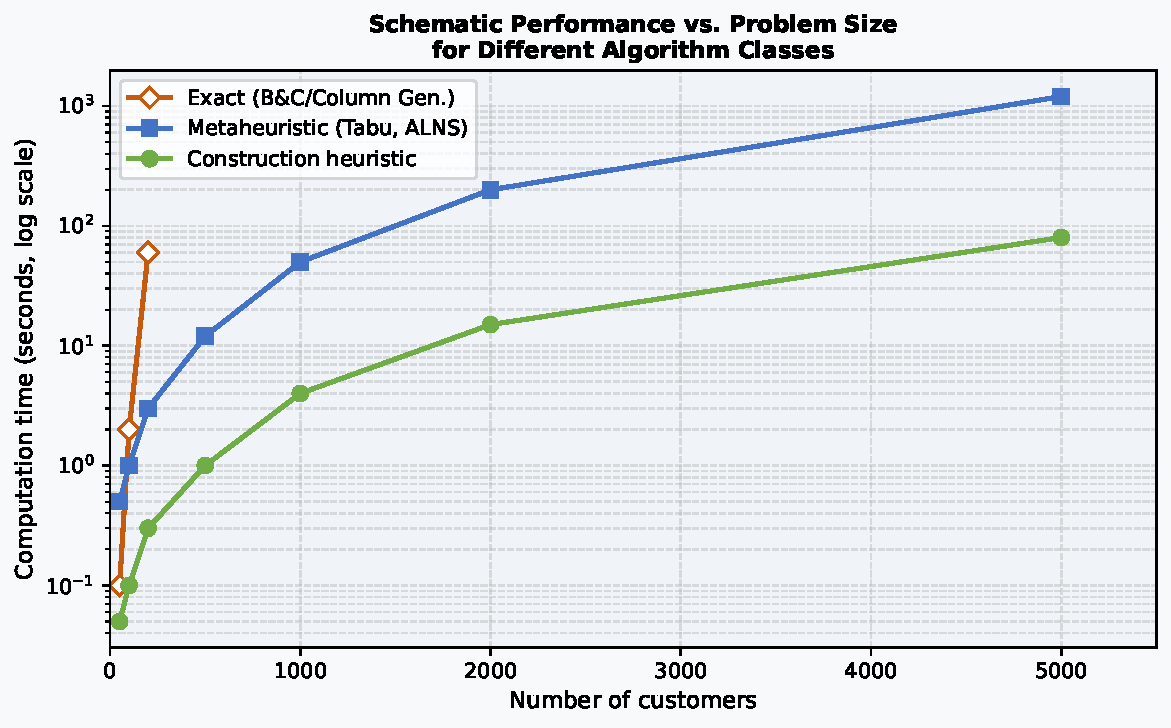
\includegraphics[width=0.80\textwidth]{fig_performance_vs_size.pdf}
    \caption{Schematic computation time as a function of problem size
             for different algorithm classes.
             Exact methods (orange) become intractable beyond $\sim$200
             customers; metaheuristics (blue) scale to thousands of customers
             in minutes; construction heuristics (green) are fastest but
             produce lower-quality solutions.}
  \end{figure}
\end{frame}

% ---- Clarke-Wright Python code (fragile frame, standalone) ----------
\begin{frame}[fragile]{Clarke-Wright Savings: Python Implementation}
  \begin{lstlisting}[caption={Clarke-Wright Savings Algorithm in Python}]
import numpy as np
from itertools import combinations

def clarke_wright(depot, customers, demands, capacity):
    """
    depot    : (x, y) coordinates of the depot
    customers: dict {id: (x, y)}
    demands  : dict {id: demand}
    capacity : vehicle capacity Q
    Returns  : list of routes, each a list of customer ids
    """
    ids = list(customers.keys())
    def dist(a, b):
        return np.linalg.norm(np.array(a) - np.array(b))

    # Step 1: compute savings s(i,j) = d(depot,i) + d(depot,j) - d(i,j)
    savings = []
    for i, j in combinations(ids, 2):
        s = (dist(depot, customers[i]) + dist(depot, customers[j])
             - dist(customers[i], customers[j]))
        savings.append((s, i, j))
    savings.sort(reverse=True)  # largest saving first

    # Step 2: initialise individual routes
    routes    = {i: [i] for i in ids}     # route key -> stop list
    route_of  = {i: i   for i in ids}     # customer  -> route key
    route_load = {i: demands[i] for i in ids}

    # Step 3: greedy merge
    for s, i, j in savings:
        ri, rj = route_of[i], route_of[j]
        if ri == rj:
            continue      # already on same route
        ri_route = routes[ri];  rj_route = routes[rj]
        if ri_route[-1] != i or rj_route[0] != j:
            # try reversed orientation
            if rj_route[-1] == j and ri_route[0] == i:
                ri_route.reverse(); rj_route.reverse()
                ri, rj = rj, ri
                ri_route, rj_route = routes[ri], routes[rj]
            else:
                continue
        if route_load[ri] + route_load[rj] > capacity:
            continue      # capacity violated
        # perform merge
        routes[ri] = ri_route + rj_route
        route_load[ri] += route_load[rj]
        del routes[rj]
        for c in rj_route:
            route_of[c] = ri

    return list(routes.values())
  \end{lstlisting}
\end{frame}

% ---- ALNS Python code (fragile frame, standalone) -------------------
\begin{frame}[fragile]{ALNS Skeleton for CVRP: Python}
  \begin{lstlisting}[caption={Adaptive Large Neighbourhood Search (ALNS) skeleton}]
import random, math, copy

def alns_cvrp(depot, customers, demands, capacity,
              n_iter=5000, q=5, T0=100.0, alpha=0.997):
    """
    ALNS for Capacitated VRP.
    alpha (alpha) : cooling rate -- temperature T decreases as T *= alpha each step.
    T0            : initial temperature (controls how often worse solutions are accepted).
    q             : number of customers removed in each destroy step.
    """
    def route_cost(routes):
        total = 0
        for r in routes:
            prev = depot
            for c in r:
                total += dist(prev, c); prev = c
            total += dist(prev, depot)
        return total

    def destroy(routes, q):
        flat = [c for r in routes for c in r]
        to_remove = set(random.sample(flat, min(q, len(flat))))
        new_routes = [[c for c in r if c not in to_remove] for r in routes]
        return [r for r in new_routes if r], list(to_remove)

    def repair(routes, removed):
        for c in removed:
            best_delta, best_r, best_pos = float('inf'), -1, -1
            for ri, r in enumerate(routes):
                if sum(demands[x] for x in r) + demands[c] > capacity:
                    continue
                for pos in range(len(r) + 1):
                    prev = depot if pos == 0 else r[pos-1]
                    nxt  = depot if pos == len(r) else r[pos]
                    delta = dist(prev,c) + dist(c,nxt) - dist(prev,nxt)
                    if delta < best_delta:
                        best_delta, best_r, best_pos = delta, ri, pos
            if best_r >= 0:
                routes[best_r].insert(best_pos, c)
            else:
                routes.append([c])
        return routes

    sol = greedy_solution(depot, customers, demands, capacity)
    best_sol, best_cost = copy.deepcopy(sol), route_cost(sol)
    T = T0
    for _ in range(n_iter):
        new_sol, removed = destroy(copy.deepcopy(sol), q)
        new_sol = repair(new_sol, removed)
        new_cost = route_cost(new_sol)
        delta = new_cost - route_cost(sol)
        # Simulated-annealing acceptance: always accept improvements;
        # accept worse solutions with probability exp(-delta/T).
        if delta < 0 or random.random() < math.exp(-delta / T):
            sol = new_sol
            if new_cost < best_cost:
                best_sol, best_cost = copy.deepcopy(sol), new_cost
        T *= alpha   # cool the temperature
    return best_sol, best_cost
  \end{lstlisting}
\end{frame}

% ---- 2-opt Python code (fragile frame, standalone) ------------------
\begin{frame}[fragile]{2-opt Local Search: Python Implementation}
  \begin{lstlisting}[caption={2-opt improvement for a single VRP route}]
import numpy as np

def two_opt(route, dist_matrix):
    """
    Improve a single route using 2-opt.
    route       : list of customer indices (depot NOT included)
    dist_matrix : 2D array where dist_matrix[i][j] is travel cost i->j

    A 2-opt move removes two edges (a->b) and (c->d) and reconnects
    as (a->c) and (b->d), reversing the segment between b and c.
    This eliminates crossing edges, always reducing total distance.
    """
    def route_cost(r):
        full = [0] + r + [0]    # 0 = depot
        return sum(dist_matrix[full[k]][full[k+1]]
                   for k in range(len(full)-1))

    improved = True
    best = route[:]
    while improved:
        improved = False
        for i in range(len(best) - 1):
            for j in range(i + 2, len(best)):
                # Reverse segment best[i+1 : j+1]
                candidate = (best[:i+1]
                             + best[i+1:j+1][::-1]
                             + best[j+1:])
                if route_cost(candidate) < route_cost(best) - 1e-10:
                    best = candidate
                    improved = True

    return best

# --- Quick demonstration ---
if __name__ == '__main__':
    np.random.seed(0)
    n = 6           # 0 = depot, 1-5 = customers
    coords = np.random.rand(n, 2) * 10
    D = np.linalg.norm(coords[:, None] - coords[None, :], axis=2)
    initial  = [1, 2, 3, 4, 5]
    improved = two_opt(initial, D)
    full_i = [0]+initial+[0];  full_o = [0]+improved+[0]
    print("Initial route :", initial,
          "  cost:", sum(D[full_i[k]][full_i[k+1]] for k in range(len(full_i)-1)))
    print("Improved route:", improved,
          "  cost:", sum(D[full_o[k]][full_o[k+1]] for k in range(len(full_o)-1)))
  \end{lstlisting}
\end{frame}

% ====================================================================
\section{Implementation, Performance, and Price}
% ====================================================================

\begin{frame}[allowframebreaks]{12.6 \; Implementation, Performance, and Price}

  This section summarises practical information about commercial VRP software
  products: what platform they run on, how they perform on standard benchmarks,
  and what they cost.

  \begin{block}{Implementation platform}
    According to the survey:
    \begin{itemize}
      \item \textbf{Almost all} commercial VRP systems are implemented in
            C++ or Java, occasionally in C\#/.NET.
            Python is rarely used for the core solver (too slow) but common
            for scripting and integration layers.
      \item \textbf{Windows} is the dominant target platform; most systems
            run natively on Windows and offer a Windows-based GUI.
      \item A growing number offer a \textbf{web-based} or
            \textbf{cloud-hosted} interface, accessible from any
            browser --- important for SaaS (Software as a Service) deployments.
      \item Linux support is available in some systems for server-side
            batch processing.
    \end{itemize}
  \end{block}

  \begin{block}{Multi-threading and performance}
    Modern VRP solvers exploit multi-core processors.
    The most advanced systems run \textbf{parallel search threads} that:
    \begin{itemize}
      \item explore different regions of the solution space simultaneously,
      \item exchange the best found solutions between threads periodically,
            and
      \item adaptively redirect search effort toward promising regions.
    \end{itemize}
    GPU (Graphics Processing Unit) computing is not yet common in
    commercial VRP tools, though academic research has demonstrated speedups
    of 10--100$\times$ for certain distance-matrix operations.
  \end{block}

  \framebreak

  \begin{block}{Solution quality benchmarks}
    Vendors are reluctant to publish benchmark results (competitive
    sensitivity), but several academic and consulting comparisons exist.
    Key findings:
    \begin{itemize}
      \item Top commercial systems typically produce solutions within
            \textbf{1--5\%} of the best known solution on Solomon's
            VRPTW benchmark instances (100 customers each).
      \item On large real-world instances (500--5000 customers),
            the gap between commercial systems can be 5--15\% in
            total distance.
      \item Computation time targets in practice: solutions for
            1000 customers in under \textbf{5--10 minutes} on a
            modern laptop.
    \end{itemize}
    The survey found that most vendors do not publish benchmark comparisons
    against competitors, making objective evaluation difficult for buyers.
  \end{block}

  \begin{block}{Pricing models}
    Commercial VRP software is sold under various pricing models:
    \begin{itemize}
      \item \textbf{Perpetual licence} --- one-time purchase fee, often
            \$10,000--\$200,000 depending on size; annual maintenance
            fees apply.
      \item \textbf{Annual subscription} --- typically \$5,000--\$50,000
            per year for a named-user or named-company licence.
      \item \textbf{SaaS / per-route pricing} --- cloud-based systems may
            charge per route optimised (e.g., \$0.10--\$1.00 per vehicle
            per day); attractive for small companies or occasional users.
      \item \textbf{Free / open-source} --- several capable open-source
            VRP solvers exist (e.g., Google OR-Tools, jsprit, OptaPlanner),
            with no licence cost but requiring technical expertise to deploy.
    \end{itemize}
  \end{block}

  \framebreak

  \begin{block}{Important future research topics (from survey)}
    Vendors identified the following as critical open problems:
    \begin{enumerate}
      \item A \textbf{general framework} for VRP that can handle
            arbitrarily complex combinations of constraints without
            requiring custom algorithm development for each new variant.
      \item Better handling of \textbf{multi-criteria optimisation}:
            simultaneously minimising cost, emissions, time, and risk.
      \item Improved \textbf{stochastic and real-time planning}:
            handling uncertainty and dynamic changes more robustly.
      \item \textbf{Load balancing} across drivers and vehicles
            for fair workload distribution.
      \item \textbf{Green routing}: minimising CO$_2$ emissions,
            considering vehicle load, road gradient, and speed profiles
            (not just distance).
    \end{enumerate}
  \end{block}

  \begin{alertblock}{Key insight}
    The VRP software market is growing rapidly, driven by e-commerce,
    same-day delivery expectations, and sustainability pressures.
    The boundary between ``routing software'' and ``logistics platform''
    is blurring: modern tools increasingly integrate fleet management,
    driver behaviour monitoring, customer communication, and
    supply chain planning.
  \end{alertblock}
\end{frame}

% ====================================================================
\section{VRP Technology Survey}
% ====================================================================

\begin{frame}[allowframebreaks]{12.7 \; VRP Technology Survey}

  The authors conducted a structured questionnaire survey of commercial VRP
  software vendors in 2013 (just before the book's publication).
  Nine companies responded, spanning Europe, North America, and Australia.
  This section presents the survey findings.

  \begin{figure}
    \centering
    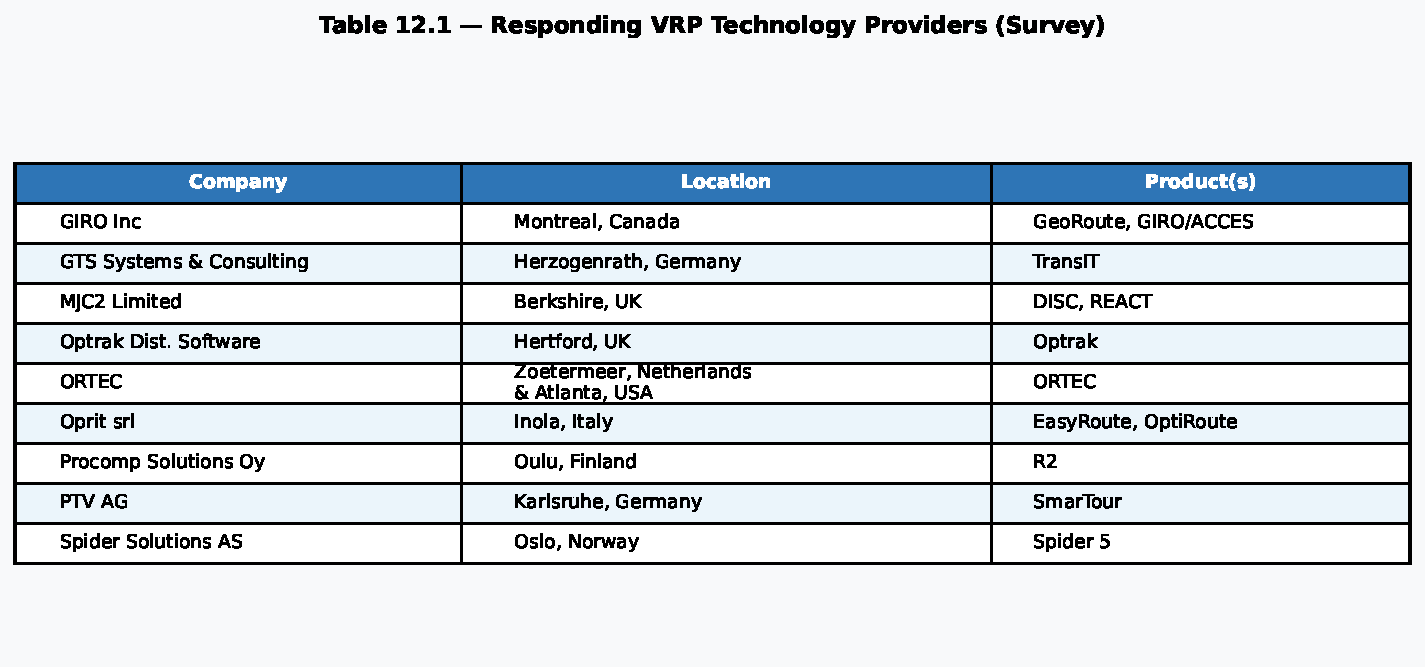
\includegraphics[width=0.88\textwidth]{fig_vendor_table.pdf}
    \caption{The nine companies that responded to the VRP technology survey
             (Table 12.1 from the book).
             They represent a diverse geographic spread and product portfolio,
             from transit planning (GIRO) to general-purpose commercial routing
             (ORTEC, PTV, Optrak).}
  \end{figure}

  \framebreak

  \begin{block}{12.7.1 \; System Architecture and Service Interfaces}
    The survey asked about how the VRP functionality is delivered to users:
    \begin{itemize}
      \item \textbf{Stand-alone desktop application} ---
            a dedicated Windows program with a full graphical user interface
            (GUI); the user installs it on a PC.
            All nine respondents offered this mode.
      \item \textbf{Decision support system with GIS integration} ---
            the routing engine is embedded in a broader platform combining
            routing, map display, and fleet management.
      \item \textbf{Web-based interface} ---
            routes accessible via browser; no local installation required.
            Five of nine respondents supported this.
      \item \textbf{API / web service} ---
            the solver is exposed as a programming interface (e.g., REST API),
            allowing customers to call the solver from their own systems
            without using the vendor's GUI.
      \item \textbf{Mobile applications} ---
            driver apps for turn-by-turn navigation and proof-of-delivery
            (electronic signature capture).
    \end{itemize}
  \end{block}

  \framebreak

  \begin{block}{12.7.2 \; Time-Dependent, Uncertainty, and Dynamics}
    \textbf{Time-dependent travel times.}
    Real road networks have time-varying travel speeds:
    motorways are fast at midnight but congested at rush hour.
    Several commercial tools support \emph{time-dependent distance matrices},
    where $d_{ij}(t)$ (d sub i,j of t) is the travel time from $i$ to $j$
    if you depart at time $t$ (t, measured in minutes from midnight or
    from the start of the planning day).
    This makes the routing problem significantly harder because feasibility
    checks must account for changing travel times as the route progresses.

    \textbf{Dynamic VRP.}
    In a dynamic setting, new customer orders arrive during the planning day.
    The system must decide whether and where to insert each new order into
    existing routes without disrupting too many planned stops.
    A key metric is the \emph{disruption cost}: how much extra distance is
    needed to accommodate the new order.
    Most commercial systems support \emph{incremental replanning}: when a new
    order arrives, they reoptimise only the affected route(s) rather than
    the entire plan.
  \end{block}

  \framebreak

  \begin{block}{12.7.3 \; Parallel Computing}
    Given the increasing availability of multi-core CPUs, the survey asked
    whether systems exploit parallelism.
    Five of the nine respondents reported using parallel computation
    in their solvers.
    Strategies include:
    \begin{itemize}
      \item \emph{Parallel independent runs}: multiple solver instances
            start from different initial solutions and run independently;
            the best result is returned.
      \item \emph{Cooperative parallel search}: threads exchange
            the best solutions found at regular intervals (similar to
            island-model evolutionary algorithms).
      \item \emph{Parallel neighbourhood evaluation}: a single search
            thread evaluates many candidate moves simultaneously across
            multiple CPU cores.
    \end{itemize}
  \end{block}

  \begin{block}{12.7.4 \; Vehicle Routing Research and Academia}
    The survey revealed a gap between academic research and commercial practice:
    \begin{itemize}
      \item Most vendors follow academic publications closely but report
            that \textbf{implementing new algorithms from scratch takes 1--3 years}
            from publication to production deployment.
      \item The academic focus on benchmark instances and distance
            minimisation does not always match real-world priorities
            (cost, time, fairness, driver satisfaction).
      \item Several vendors mentioned that academic VRP tools
            (research prototypes) are rarely directly usable
            in production; they require re-engineering for robustness,
            scalability, and constraint richness.
      \item \textbf{Open source as a complement}: some vendors incorporate
            open-source components (e.g., graph libraries, GIS tools) while
            keeping the core solver proprietary.
    \end{itemize}
  \end{block}

  \framebreak

  \begin{block}{12.7.5 \; Important Future Research Topics (Survey Responses)}
    Vendors were asked: ``What are the most important open research problems?''
    Top answers:
    \begin{enumerate}
      \item \textbf{Generic multi-constraint solver framework} ---
            a single algorithmic framework that handles any combination of
            VRP constraints without manual tuning.
      \item \textbf{Better integration of uncertainty} ---
            stochastic demands, uncertain travel times, cancellations.
      \item \textbf{Real-time replanning at scale} ---
            reoptimise 1000+ vehicles within seconds when new orders arrive.
      \item \textbf{CO$_2$ and emission minimisation} ---
            green routing with fuel consumption models (not just distance).
      \item \textbf{Machine learning for parameter setting} ---
            automatically tune algorithm parameters (e.g., tabu tenure,
            destroy size in ALNS) based on instance characteristics.
      \item \textbf{Multi-modal routing} ---
            combining road vehicles, rail, and urban last-mile delivery.
    \end{enumerate}
  \end{block}

  \begin{alertblock}{Key takeaway from the survey}
    The gap between what commercial software can do and what the academic
    literature has achieved is narrowing, but it has not closed.
    The most successful vendors are those who invest in bridging this gap:
    hiring researchers, publishing benchmark results, and collaborating
    with universities.
  \end{alertblock}
\end{frame}

% ====================================================================
\section{New and Emerging Technologies}
% ====================================================================

\begin{frame}[allowframebreaks]{12.8 \; New and Emerging Technologies}

  The VRP software landscape is being reshaped by several technology waves
  that were emerging at the time of writing (2013--2014) and have since
  become mainstream.

  \begin{figure}
    \centering
    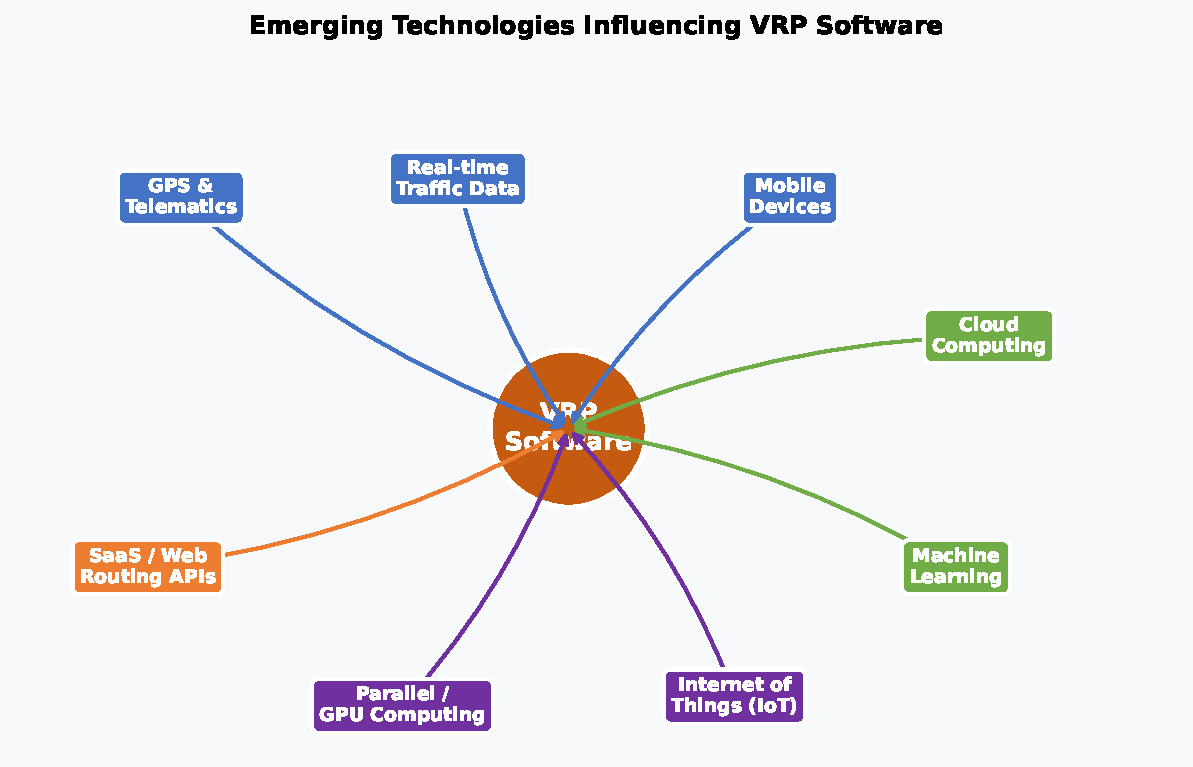
\includegraphics[width=0.80\textwidth]{fig_emerging_technologies.pdf}
    \caption{Emerging technologies influencing VRP software.
             Each node represents a technology trend that is changing
             how routing problems are modelled, solved, or deployed.}
  \end{figure}

  \framebreak

  \begin{block}{GPS and telematics}
    \textbf{GPS (Global Positioning System)} tracking provides real-time
    location data for every vehicle in a fleet.
    \textbf{Telematics} extends this with data on:
    \begin{itemize}
      \item vehicle speed, acceleration, and braking (driver behaviour),
      \item engine diagnostics (fuel consumption, idle time),
      \item refrigeration unit temperature (for cold chain), and
      \item door open/close events (proof of delivery).
    \end{itemize}
    This data enables:
    \begin{itemize}
      \item \textbf{Real-time progress monitoring}: dispatchers see which
            stops have been completed and which are delayed.
      \item \textbf{ETA (Estimated Time of Arrival) updates}: customers
            receive automated notifications when the driver is nearby.
      \item \textbf{Route adherence monitoring}: alerts when a driver
            deviates significantly from the planned route.
      \item \textbf{Historical analysis}: actual vs.\ planned performance
            data used to improve future planning models.
    \end{itemize}
  \end{block}

  \framebreak

  \begin{block}{Real-time traffic integration}
    Modern routing systems can ingest \textbf{live traffic data} (from
    sources such as HERE Traffic, Google Traffic, or proprietary probe
    vehicles) to update travel-time estimates during the day.
    This enables \emph{traffic-aware routing}: the system avoids congested
    roads when building initial routes and replans when unexpected delays
    develop.

    The technical challenge is that a VRP optimiser typically builds routes
    using a \emph{fixed} distance/time matrix computed before the planning
    day begins.
    Incorporating real-time traffic requires:
    \begin{itemize}
      \item a \emph{rolling time-dependent matrix} that is updated periodically
            (e.g., every 15 minutes), and
      \item a \emph{fast replanning algorithm} that can reoptimise the
            remaining portions of routes within seconds.
    \end{itemize}
  \end{block}

  \begin{block}{Mobile devices and driver apps}
    Smartphones and tablet computers have transformed driver communication.
    Instead of a paper manifest, drivers receive their routes on a mobile app
    that provides:
    \begin{itemize}
      \item turn-by-turn navigation,
      \item electronic proof of delivery (signature capture, photo),
      \item two-way communication with the dispatcher,
      \item automatic stop completion recording (geo-fence triggers), and
      \item real-time updates when the planned route changes.
    \end{itemize}
  \end{block}

  \framebreak

  \begin{figure}
    \centering
    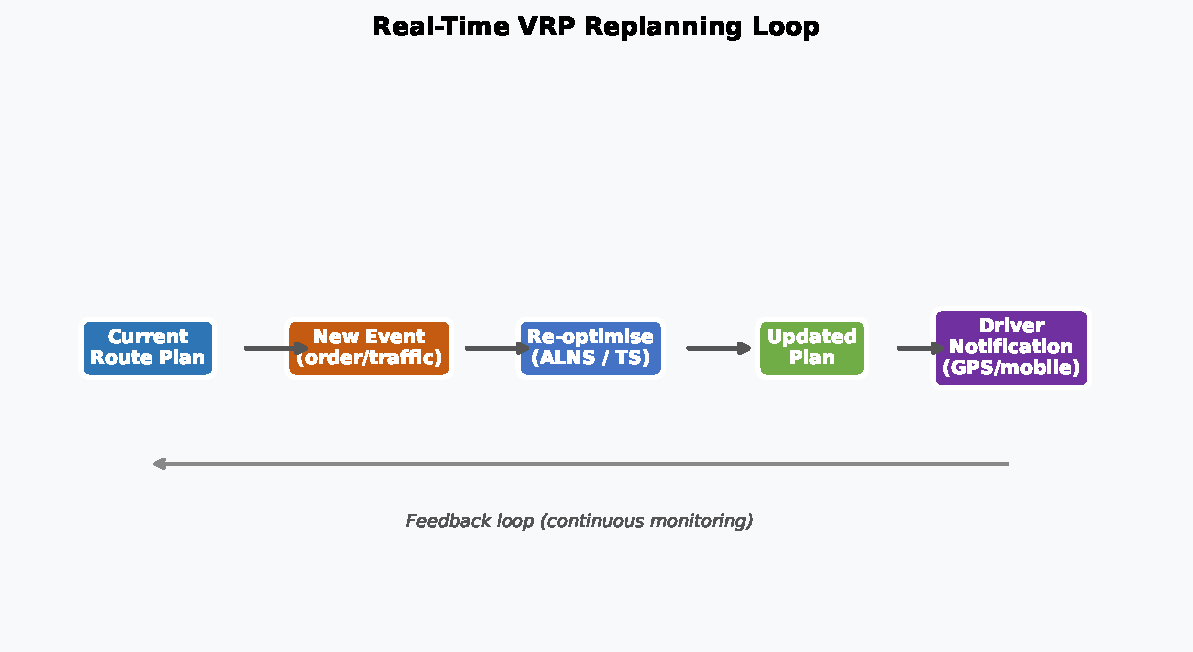
\includegraphics[width=0.83\textwidth]{fig_realtime_loop.pdf}
    \caption{The real-time VRP replanning loop.
             A new event (new order, traffic jam, vehicle breakdown) triggers
             the optimiser to update the affected routes.
             The updated plan is sent to the driver via GPS/mobile device.
             This loop runs continuously throughout the day.}
  \end{figure}

  \framebreak

  \begin{block}{Cloud computing and SaaS}
    \textbf{Cloud computing} has changed the economics of VRP software:
    \begin{itemize}
      \item \textbf{No upfront infrastructure cost}: the vendor runs the
            solver on cloud servers (AWS, Azure, GCP); the customer pays
            a subscription.
      \item \textbf{Scalability on demand}: a cloud-based solver can spin
            up additional compute nodes for large daily planning runs
            and release them when done.
      \item \textbf{Automatic updates}: customers always run the latest
            version without manual installation.
      \item \textbf{Integration via API}: other IT systems (ERP, e-commerce
            platform, TMS) can call the routing engine directly via a
            REST API, enabling fully automated order-to-route workflows.
    \end{itemize}

    \textbf{SaaS (Software as a Service)} VRP platforms available in 2014
    included early versions of products like Google Maps Platform routing
    and various startup offerings.
    By 2024, the market includes dozens of cloud-native VRP services.
  \end{block}

  \begin{figure}
    \centering
    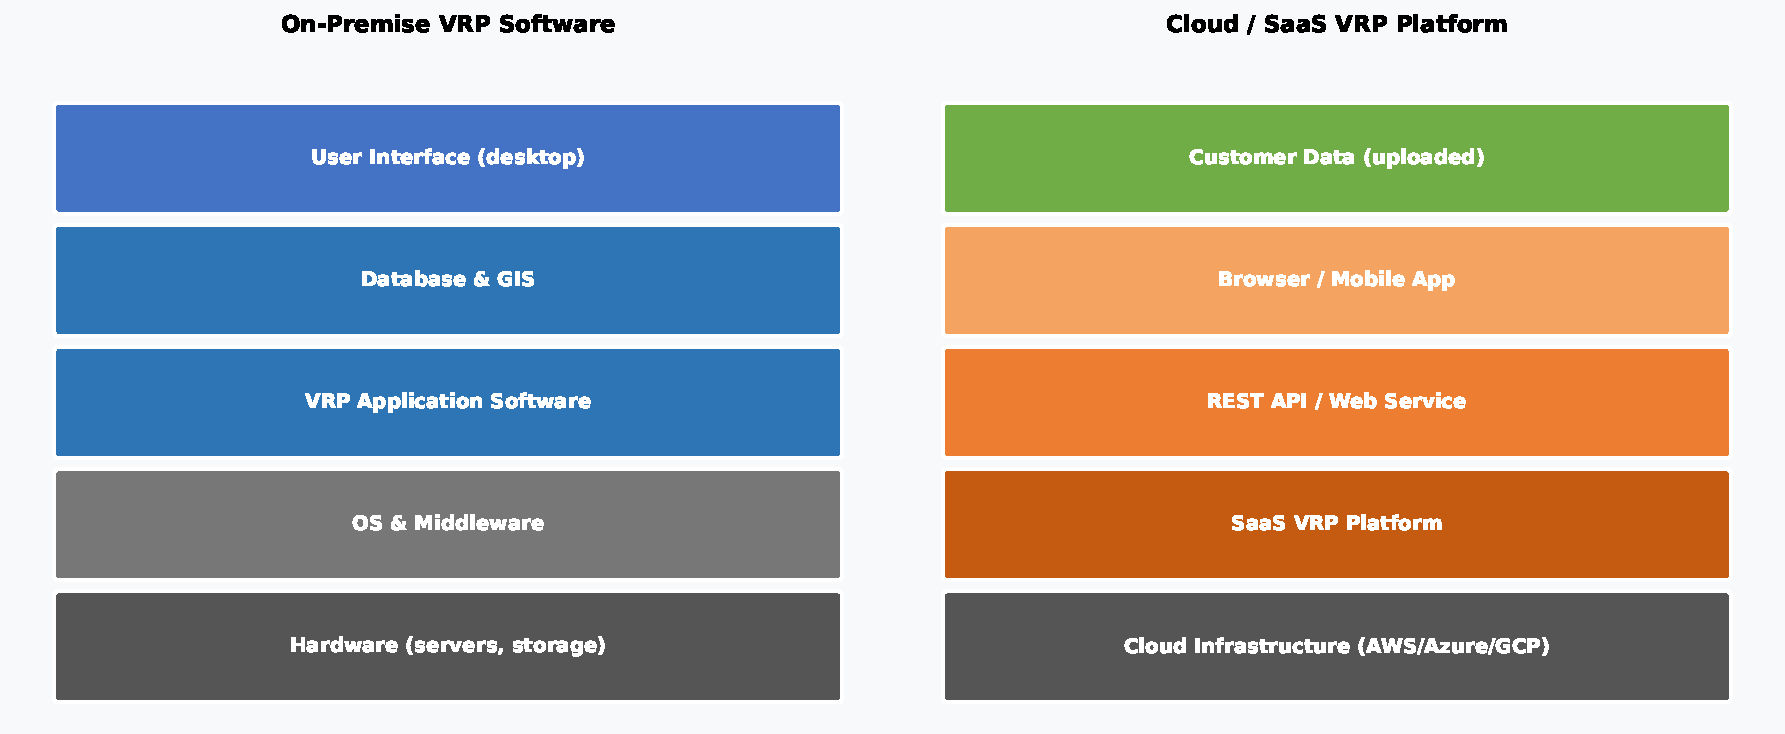
\includegraphics[width=0.86\textwidth]{fig_saas_vs_onpremise.pdf}
    \caption{On-premise (left) vs.\ cloud/SaaS (right) VRP software
             architecture.
             On-premise requires the customer to own and maintain hardware
             and software; cloud/SaaS moves infrastructure management to
             the vendor, with the customer accessing the system via browser
             or API.}
  \end{figure}

  \framebreak

  \begin{block}{Machine learning and data-driven VRP}
    At the time of the book's writing, machine learning (ML) was beginning
    to influence VRP through:
    \begin{itemize}
      \item \textbf{Demand forecasting}: predicting how many orders each
            customer will place on a given day, enabling proactive fleet
            sizing.
      \item \textbf{Travel time prediction}: using historical GPS data to
            build time-of-day speed profiles for each road segment.
      \item \textbf{Parameter tuning}: using ML to set metaheuristic
            parameters (e.g., ALNS destroy size, tabu tenure) based on
            instance features.
    \end{itemize}
    Since 2014, deep learning has further advanced these applications,
    and \emph{neural combinatorial optimisation} (using neural networks
    to directly construct VRP solutions) has emerged as an active
    research direction.
  \end{block}

  \begin{block}{The Internet of Things (IoT)}
    Smart sensors on vehicles, pallets, and packages create a stream of
    real-time data that enriches routing decisions:
    \begin{itemize}
      \item Pallet weight sensors confirm actual loads, triggering
            replanning if a vehicle is over capacity.
      \item Temperature sensors in cold-chain vehicles trigger alerts
            if the refrigeration unit fails during a route.
      \item Package RFID (Radio Frequency Identification) tags enable
            automatic delivery confirmation without driver action.
    \end{itemize}
  \end{block}
\end{frame}

% ====================================================================
\section{The Future of the VRP Business}
% ====================================================================

\begin{frame}[allowframebreaks]{12.9 \; The Future of the VRP Business}

  The authors conclude with a forward-looking perspective on where the
  VRP software industry is heading.
  Several structural trends were reshaping the market in 2013--2014 and
  have since accelerated.

  \begin{block}{New delivery modes require new VRP models}
    The traditional VRP deals with human-driven trucks and vans.
    Emerging delivery modes that require new modelling approaches include:
    \begin{itemize}
      \item \textbf{Electric vehicles (EVs)}: limited range, charging time
            constraints, availability of charging stations --- leading to
            the \emph{Green VRP} and \emph{Electric VRP} (E-VRP) variants.
      \item \textbf{Autonomous delivery vehicles}: self-driving trucks and
            vans remove the driver constraint but introduce new safety and
            regulatory constraints.
      \item \textbf{Delivery drones (UAVs)}: used for last-mile delivery
            in rural or congested urban areas; modelled as the
            \emph{truck-and-drone routing problem}.
      \item \textbf{Cargo bikes}: zero-emission last-mile delivery in
            city centres; limited by payload and range.
    \end{itemize}
  \end{block}

  \framebreak

  \begin{block}{Market consolidation and platform competition}
    The VRP software market in 2014 comprised dozens of small specialist
    vendors.
    Since then, several consolidation trends have occurred:
    \begin{itemize}
      \item Large logistics platform companies (e.g., Oracle, SAP,
            Trimble, MercuryGate) have acquired specialist routing vendors.
      \item Technology giants (Google, Amazon, Uber) have entered the
            space with their own routing platforms, primarily for
            their own operations but increasingly offered as services.
      \item \textbf{Open-source tools} such as Google OR-Tools have
            become sophisticated enough for many real-world applications,
            putting competitive pressure on commercial vendors.
    \end{itemize}
  \end{block}

  \begin{block}{The role of open-source VRP solvers}
    Open-source VRP frameworks available as of 2014 and beyond:
    \begin{itemize}
      \item \textbf{Google OR-Tools} (C++/Python/Java) ---
            includes CVRP, VRPTW, and pickup-and-delivery solvers;
            actively maintained; widely used in industry.
      \item \textbf{jsprit} (Java) ---
            a flexible, metaheuristic-based VRP toolkit using ALNS;
            supports many VRP variants.
      \item \textbf{OptaPlanner} (Java) ---
            a constraint satisfaction and planning framework with
            VRP support.
      \item \textbf{VeRoLog Solver Challenge tools} ---
            academic solvers released as part of EURO working group
            competitions.
    \end{itemize}
    Open-source tools are particularly valuable for research, prototyping,
    and small-scale deployments.
    They lack the map integration, user interfaces, and enterprise support
    of commercial products.
  \end{block}

  \framebreak

  \begin{block}{Sustainability and green logistics}
    Reducing the environmental impact of freight is a growing priority
    for businesses and regulators.
    VRP software is evolving to support:
    \begin{itemize}
      \item \textbf{CO$_2$ minimisation as an objective} ---
            not just distance, but actual fuel-based emissions
            (which depend on load, speed, terrain, and vehicle type).
      \item \textbf{Multi-objective optimisation} ---
            presenting planners with a \emph{Pareto frontier} of
            solutions trading off cost vs.\ emissions vs.\ time.
      \item \textbf{Regulatory compliance} ---
            low-emission zones in cities require certain vehicle types;
            time-of-day access restrictions in urban areas.
    \end{itemize}
  \end{block}

  \begin{alertblock}{Key insight: the future of VRP technology}
    The core optimisation problem (VRP) is unlikely to be ``solved'' in
    any absolute sense --- new business models, vehicle types, and
    constraints continually create new variants.
    The competitive advantage of VRP software vendors will increasingly
    come from: (a) the breadth and richness of their constraint models,
    (b) real-time integration with IoT, traffic, and mobile data, and
    (c) the quality of the human--machine interface that allows planners
    to trust, understand, and effectively use the automated routes.
  \end{alertblock}
\end{frame}

% ====================================================================
\section{Summary and Conclusions}
% ====================================================================

\begin{frame}[allowframebreaks]{12.10 \; Summary and Conclusions}

  This chapter has provided a comprehensive survey of the VRP software
  technology landscape.
  Here we collect the main lessons.

  \begin{block}{What makes a good VRP software product?}
    Based on the survey and analysis, a high-quality VRP software product:
    \begin{enumerate}
      \item \textbf{Models the real problem accurately} ---
            supports the constraint types (time windows, multiple capacities,
            compatibility, driving regulations) that arise in the target
            industry.
      \item \textbf{Produces high-quality solutions efficiently} ---
            within 1--5\% of optimal for standard benchmarks,
            in practically acceptable computation times
            (seconds to minutes for operational planning).
      \item \textbf{Integrates seamlessly} ---
            reads data from existing ERP/TMS systems, uses current
            digital maps, and exports results in usable formats.
      \item \textbf{Provides an effective user interface} ---
            planners can see, understand, and manually adjust routes;
            the system supports human--machine interaction, not just
            fully automated black-box optimisation.
      \item \textbf{Scales to operational size} ---
            handles 1,000--10,000 customer visits per day on
            standard hardware, with acceptable response times.
      \item \textbf{Embraces emerging technologies} ---
            supports real-time data (GPS, traffic), mobile dispatch,
            and cloud deployment.
    \end{enumerate}
  \end{block}

  \framebreak

  \begin{block}{Algorithm choices in practice}
    The dominant algorithmic approach in commercial VRP software is
    \textbf{metaheuristics} (especially Tabu Search and ALNS),
    supplemented by fast construction heuristics for initial solutions.
    Exact methods are used only for small sub-problems.
    The most capable systems combine:
    \begin{itemize}
      \item a Clarke-Wright or nearest-neighbour \textbf{construction phase},
      \item a Tabu Search or ALNS \textbf{improvement phase},
      \item a \textbf{feasibility repair mechanism} to handle
            constraint violations encountered during search, and
      \item \textbf{parallel multi-start}: multiple independent solver
            threads starting from different initial solutions.
    \end{itemize}
  \end{block}

  \begin{block}{The research-practice gap}
    Academic VRP research often focuses on:
    \begin{itemize}
      \item a single, well-defined problem variant,
      \item distance minimisation as the sole objective,
      \item small to medium benchmark instances, and
      \item theoretical performance guarantees.
    \end{itemize}
    Commercial practice requires:
    \begin{itemize}
      \item arbitrary combinations of constraints,
      \item multi-objective (cost, time, emissions, fairness),
      \item very large instances (1,000s of customers), and
      \item robustness to data errors and user overrides.
    \end{itemize}
    Closing this gap is the central long-term challenge for the field.
  \end{block}

  \framebreak

  \begin{block}{Key facts from the technology survey}
    \begin{itemize}
      \item Nine leading vendors responded, spanning Europe and North America.
      \item \textbf{All} supported time windows, multi-depot, and capacity constraints.
      \item \textbf{Most} supported heterogeneous fleets, priorities, and
            pickup-and-delivery.
      \item \textbf{Fewer} supported stochastic demands, split deliveries,
            and full driving-hours regulations.
      \item \textbf{Five of nine} used parallel computing in their solvers.
      \item \textbf{Most} planned to adopt cloud/SaaS delivery models within
            three years of the survey (i.e., by 2016--2017).
      \item Pricing ranged from free (open-source) to \$200,000+ for
            enterprise perpetual licences.
    \end{itemize}
  \end{block}

  \begin{alertblock}{Final takeaway}
    Vehicle routing optimisation has matured from a purely academic topic
    into a multi-billion-dollar software industry.
    The most impactful future research directions are those that directly
    address real business needs: handling uncertainty and dynamics in
    real time, supporting green and multi-modal logistics, and developing
    human-centred interfaces that build planner trust in automated solutions.
  \end{alertblock}

  \framebreak

  \begin{block}{Selected Bibliography (key references from Chapter 12)}
    \footnotesize
    \begin{itemize}
      \item \textbf{Clarke \& Wright (1964)}: ``Scheduling of vehicles from
            a central depot to a number of delivery points.''
            \emph{Operations Research}, 12, 568--581.
            --- Original savings algorithm.
      \item \textbf{Ropke \& Pisinger (2006)}: ``An adaptive large neighbourhood
            search heuristic for the pickup and delivery problem with time windows.''
            \emph{Transportation Science}, 40(4), 455--472.
            --- ALNS framework.
      \item \textbf{Glover (1986)}: ``Future paths for integer programming and
            links to artificial intelligence.'' \emph{Computers \& OR}, 13, 533--549.
            --- Original Tabu Search.
      \item \textbf{Taillard et al.\ (1997)}: ``A tabu search heuristic for the
            vehicle routing problem with soft time windows.''
            \emph{Transportation Science}, 31, 170--186.
      \item \textbf{Vidal et al.\ (2013)}: ``A hybrid genetic algorithm with
            adaptive diversity management for a large class of vehicle routing
            problems with time-windows.''
            \emph{Computers \& OR}, 40, 475--489.
      \item \textbf{Desaulniers, Desrosiers \& Solomon (2002)}:
            \emph{Column Generation}. Springer.
      \item \textbf{Halse (1992)}: ``Modelling and solving complex vehicle
            routing problems.'' PhD thesis, DTU.
      \item \textbf{Solomon (1987)}: ``Algorithms for the vehicle routing and
            scheduling problems with time window constraints.''
            \emph{Operations Research}, 35, 254--265.
            --- Standard VRPTW benchmark instances.
    \end{itemize}
  \end{block}
\end{frame}

% ====================================================================
\begin{frame}[allowframebreaks]{End of Chapter 12}
  \centering
  \vspace{1.5cm}
  {\Large\bfseries Chapter 12 Complete}\\[1em]
  {\large Software Tools and Emerging Technologies\\
  for Vehicle Routing and Transportation}\\[2em]
  \begin{block}{Chapter covered}
    \begin{itemize}
      \item Architecture of VRP routing software systems
      \item Input/output, GIS integration, and data formats
      \item Supported VRP model properties and constraint types
      \item Embedded algorithms: Clarke-Wright, Tabu Search, ALNS, 2-opt
      \item Implementation platforms, performance, and pricing
      \item Survey results from 9 leading commercial vendors
      \item Emerging technologies: GPS, telematics, cloud, IoT, ML
      \item Future directions: EVs, drones, green logistics, SaaS
    \end{itemize}
  \end{block}
\end{frame}

\end{document}
